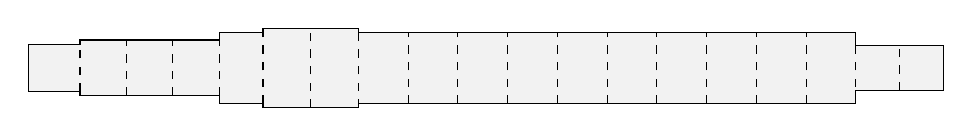
\begin{tikzpicture}[scale=\linewidth/120cm]

    % shaft
    \draw[fill=gray!10] (0,-2.975) -- (6.5,-2.975) -- (6.5,-3.5) -- (24.0, -3.5) -- (24.0, -4.485) -- (29.5, -4.485) -- (29.5, -4.985) -- (41.5, -4.985) -- (41.5, -4.485) -- (104.0, -4.485) -- (104.0, -2.8225) -- (115.0, -2.8225) -- (115.0, 2.8225) -- (104.0, 2.8225) -- (104.0, 4.485) -- (41.5, 4.485) -- (41.5, 4.985) -- (29.5, 4.985) -- (29.5, 4.485) -- (24.0, 4.485) -- (24.0, 3.5) -- (6.5, 3.5) -- (6.5, 2.975) -- (0, 2.975) -- cycle;

    % Devisions
    \draw[dashed] (6.5, -2.975) -- (6.5, 2.975);

    \draw[dashed] (12.3, -3.5) -- (12.3, 3.5);
    \draw[dashed] (18.1, -3.5) -- (18.1, 3.5);
    \draw[dashed] (24, -3.5) -- (24, 3.5);

    \draw[dashed] (29.5, -4.485) -- (29.5, 4.485);

    \draw[dashed] (35.5, -4.985) -- (35.5, 4.985);
    \draw[dashed] (41.5, -4.985) -- (41.5, 4.985);

    \draw[dashed] (47.75, -4.485) -- (47.75, 4.485);
    \draw[dashed] (54, -4.485) -- (54, 4.485);
    \draw[dashed] (60.25, -4.485) -- (60.25, 4.485);
    \draw[dashed] (66.5, -4.485) -- (66.5, 4.485);
    \draw[dashed] (72.75, -4.485) -- (72.75, 4.485);
    \draw[dashed] (79, -4.485) -- (79, 4.485);
    \draw[dashed] (85.25, -4.485) -- (85.25, 4.485);
    \draw[dashed] (91.5, -4.485) -- (91.5, 4.485);
    \draw[dashed] (97.75, -4.485) -- (97.75, 4.485);
    \draw[dashed] (104, -4.485) -- (104, 4.485);

    \draw[dashed] (109.5, -2.8225) -- (109.5, 2.8225);
    

\end{tikzpicture}